%%=============================================================================
%% Conclusie
%%=============================================================================

\chapter{Proof of Concept}%
\label{ch:Proof of Concept}

% TODO: Trek een duidelijke conclusie, in de vorm van een antwoord op de
% onderzoeksvra(a)g(en). Wat was jouw bijdrage aan het onderzoeksdomein en
% hoe biedt dit meerwaarde aan het vakgebied/doelgroep? 
% Reflecteer kritisch over het resultaat. In Engelse teksten wordt deze sectie
% ``Discussion'' genoemd. Had je deze uitkomst verwacht? Zijn er zaken die nog
% niet duidelijk zijn?
% Heeft het onderzoek geleid tot nieuwe vragen die uitnodigen tot verder 
%onderzoek?

\section{\IfLanguageName{dutch}{Ontwikkeling van de mobiele app}{Development mobile app}}%
\label{sec:ontwikkeling mobiele app}

Om de onderzoeksvraag van deze bachelorproef te kunnen beantwoorden werden een Python web server en een  iOS app ontwikkeld als proof of concept. Deze app maakt in de eerste plaats het elektriciteitsverbruik en de stroomproductie van de zonnepanelen inzichtelijk. Daarnaast zal de app via de toepassing van machine learning de elektriciteitsproductie van de volgende dag voorspellen. Deze voorspelling zal dan door de app gebruikt worden om de inschakeling van twee slimme stekkers te programmeren indien er voldoende stroomproductie voorspeld wordt.

\subsection{\IfLanguageName{dutch}{Digitale elektriciteitsmeter uitlezen}{Reading out digital electricitymeter}}%
\label{sec:Digitale elektriciteitsmeter uitlezen}

Een mobiele app die het elektriciteitsverbruik wil bijsturen en beter spreiden zal de gebruiker ervan allereerst inzicht moeten geven in zijn of haar verbruik. Om de verbruiksgegevens te ontsluiten moet de digitale elektriciteitsmeter uitgelezen worden via de P1-poort. Hiervoor zijn verschillende mogelijkheden, van een dongle tot kleine toestellen die via een kabel met de P1-poort kunnen verbonden worden. Voor dit onderzoek is er gekozen voor een Raspberry Pi 5 minicomputer om de digitale meter uit te lezen. Deze singleboardcomputer die gebaseerd is op een ARM processor en de Linuxdistributie Ubuntu als besturingssysteem heeft, biedt meer mogelijkheden dan enkel het uitlezen van data. Omdat het verbruik ervan zeer laag is, kan dit toestel bovendien continu ingeschakeld blijven. Daarnaast heeft de Raspberry Pi wifi-ondersteuning zodat deze kan verbonden worden met het wifi-netwerk van de woning die als testomgeving gebruikt wordt. Dit maakt het mogelijk om een webserver op te zetten en meteen ook de omvormer van de zonnepanelen van de woning via het wifi-netwerk uit te lezen met de Raspberry Pi (zie volgende sectie). In de testwoning bevindt de digitale elektriciteitsmeter zich namelijk in de kelder, terwijl de omvormer van de zonnepanelen zich op zolder bevindt. Een situatie die wel vaker voorkomt en op deze manier kan worden opgelost.

\begin{figure}[h!]
    \centering
    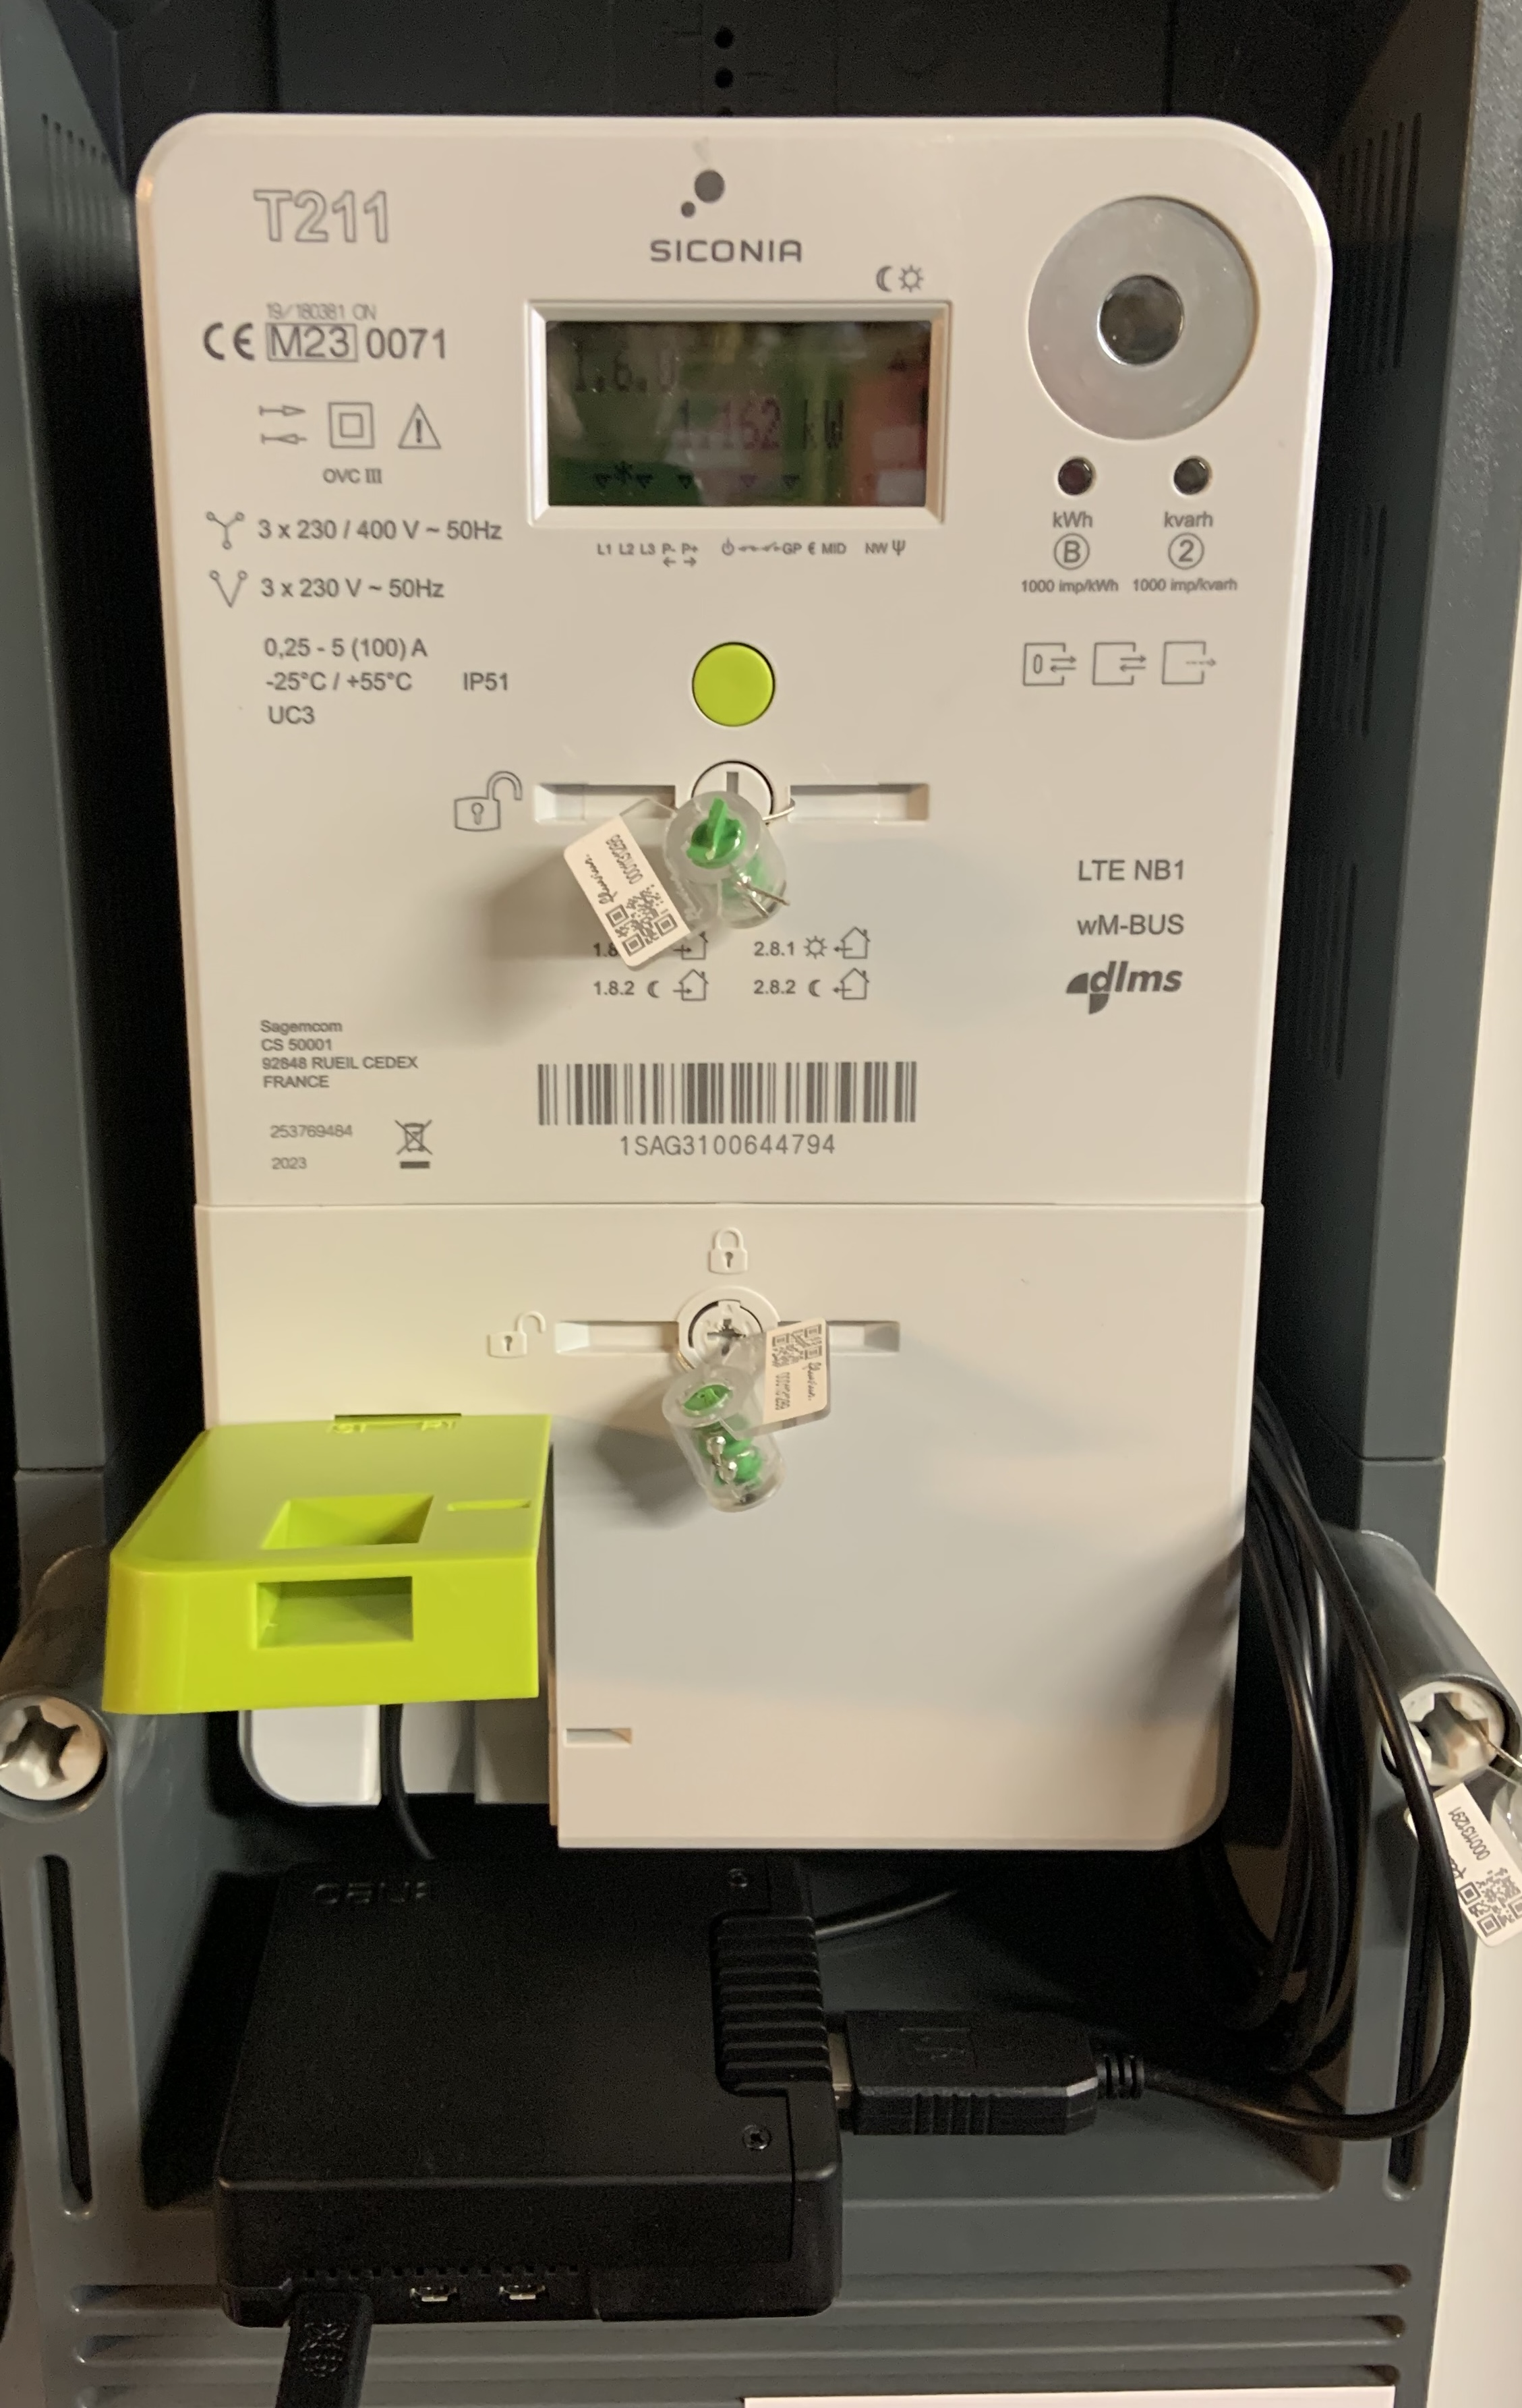
\includegraphics[width=7cm]{TestSetup} \hspace{0.7cm}
    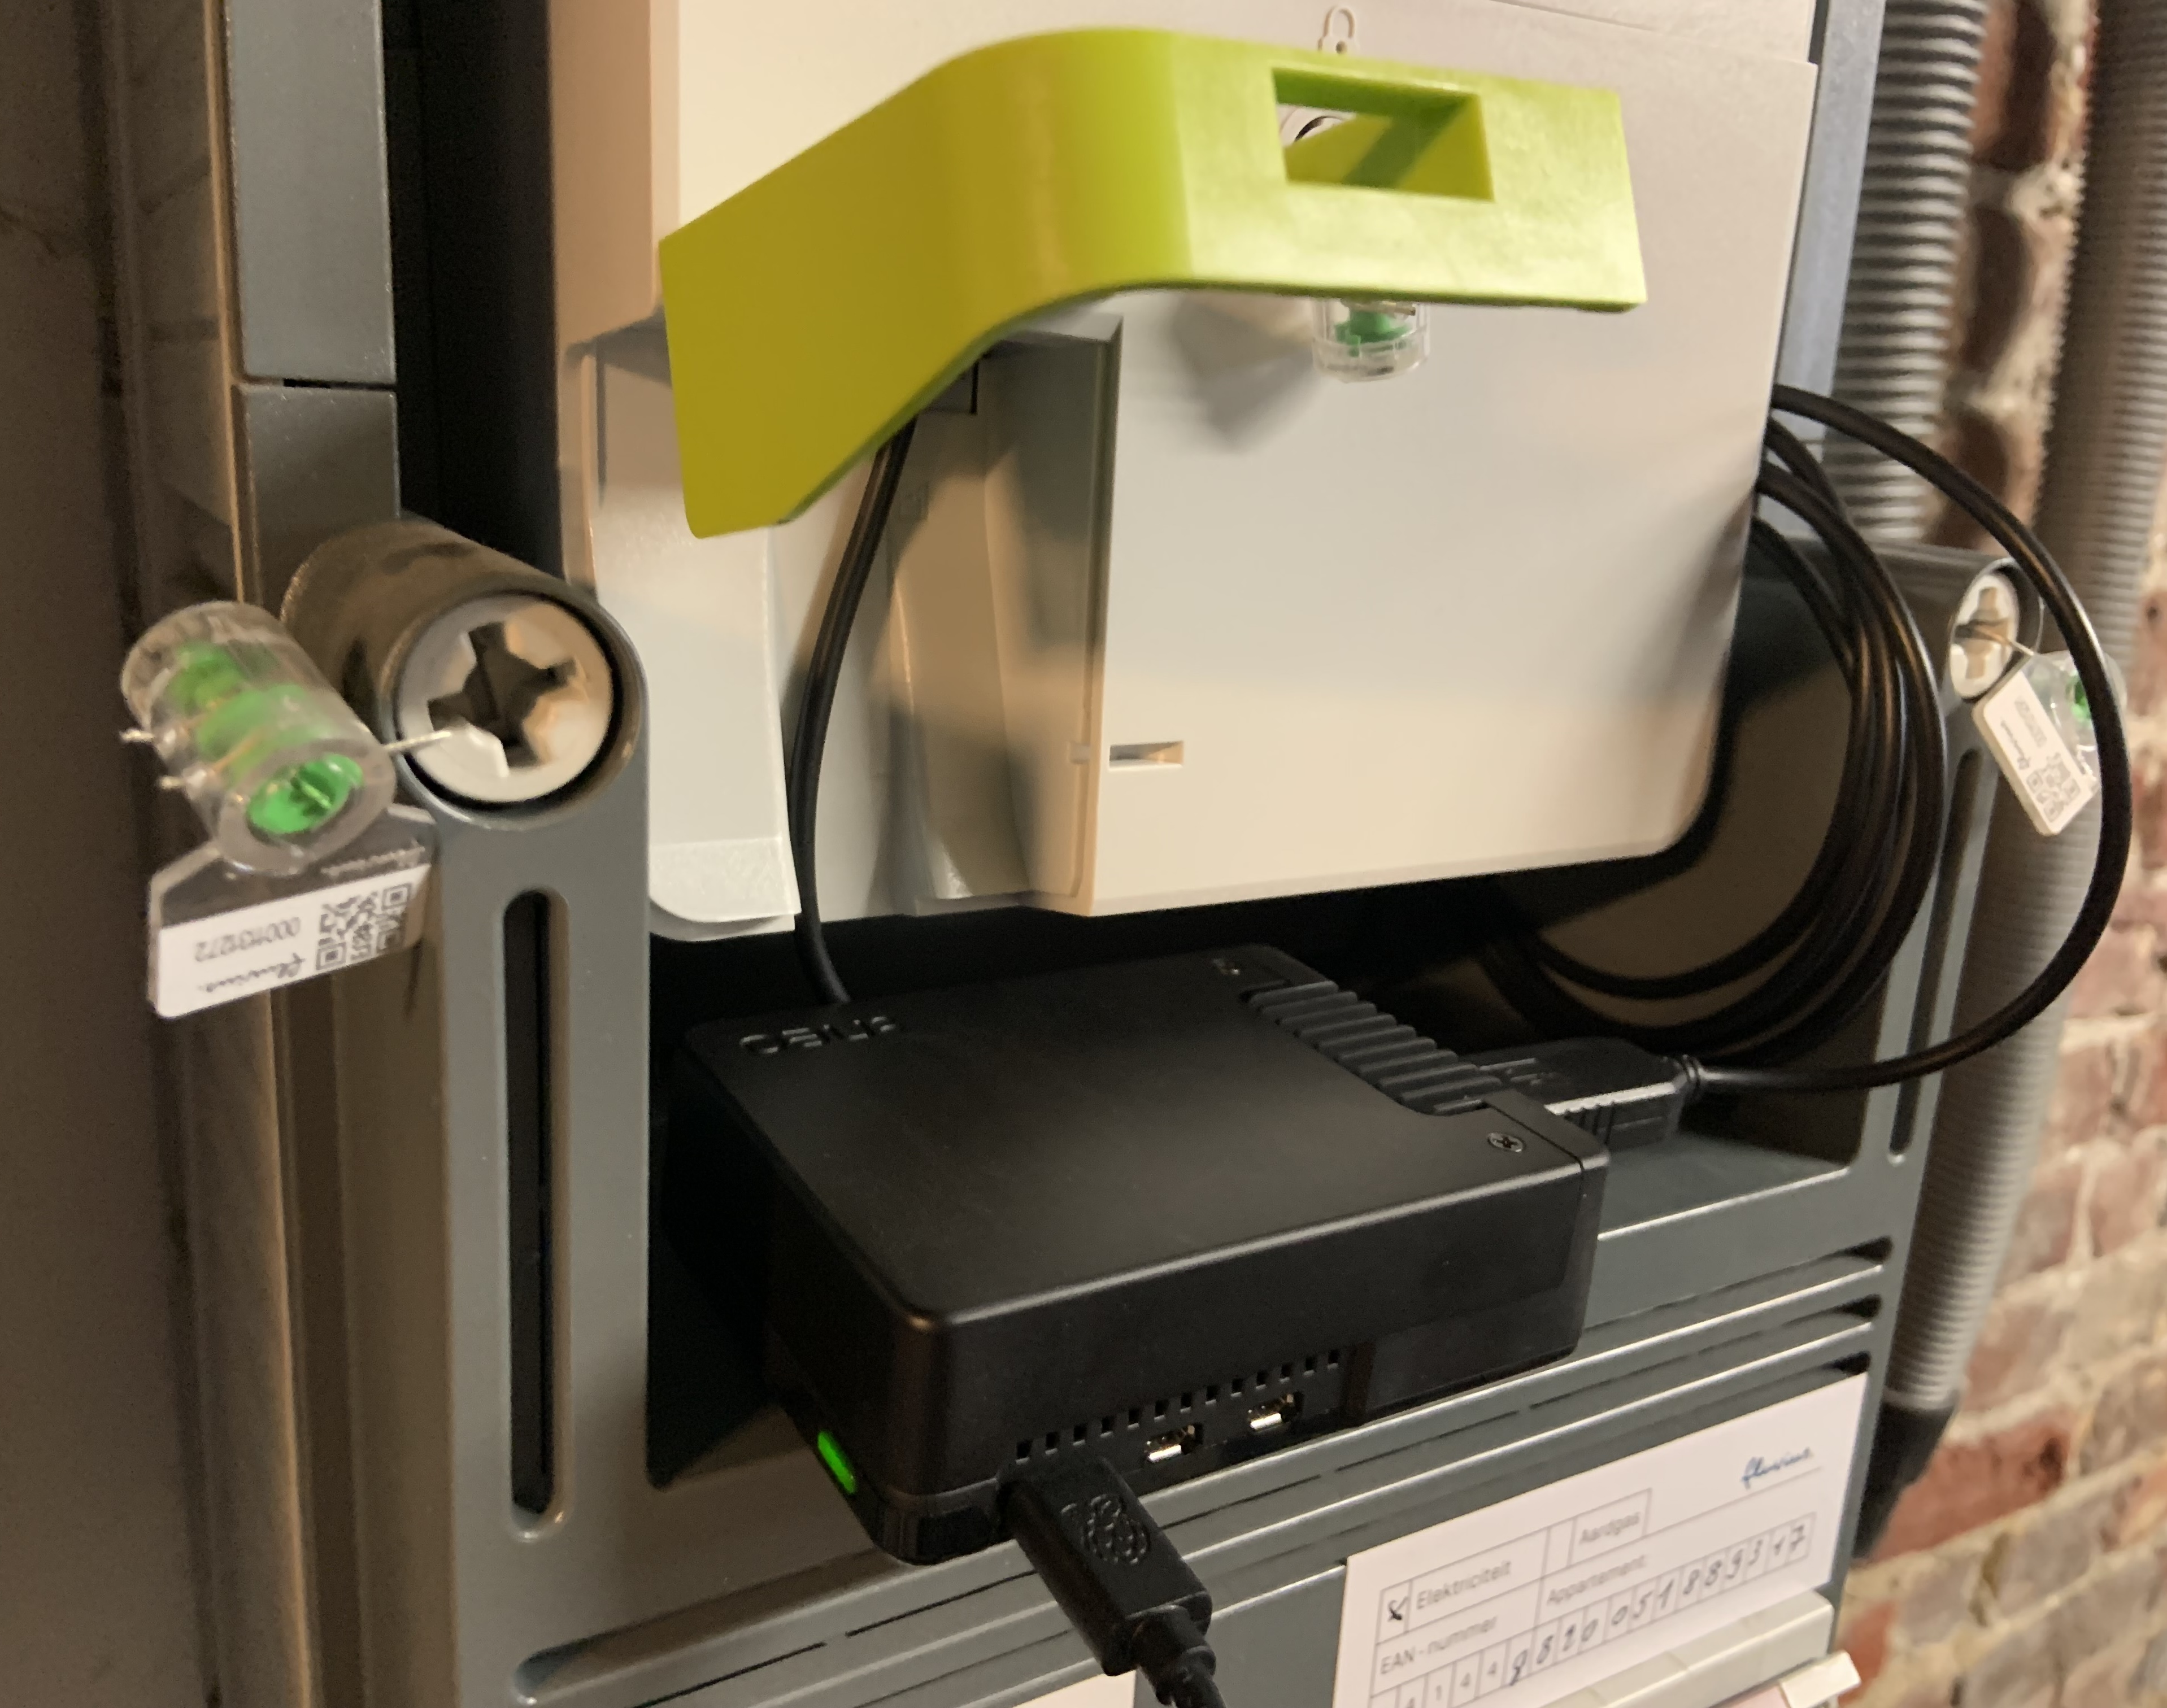
\includegraphics[width=7cm]{RPi5}
    \caption{Testopstelling: Raspberry Pi 5 via een RS422 serieel naar USB kabel aangesloten op een digitale elektriciteitsmeter.}
\end{figure}

\subsubsection{Opslag uitgelezen elektriciteitsdata}

Nadat de Raspberry Pi via de juiste kabel op de P1-poort werd aangesloten, kon de data van de digitale elektriciteitsmeter via een Python script worden uitgelezen. Hiervoor werd een bestaand Python script uitgebreid \autocite{Depuydt2021}. Het bestaande script voorzag enkel in het uitprinten van de uitgelezen data in de console. Om de uitgelezen elektriciteitsdata later via een app te kunnen weergeven moest deze data worden weggeschreven naar een databank. Omdat de data via de P1-poort per seconde uitgelezen wordt, werd geopteerd voor InfluxDB. Deze NoSQL-databank is speciaal ontwikkeld voor time-series en is binnen bepaalde (ruime) grenzen gratis te gebruiken \autocite{Balis2017} en  \autocite{Struckov2019}. Het Python script werd tenslotte opgezet als een achtergrond service via de systeem manager voor Linux 'systemctl/systemd', zodat het voortdurend blijft uitgevoerd worden.

\subsection{\IfLanguageName{dutch}{Omvormer zonnepanelen uitlezen}{Reading out power converter PV system}}%
\label{sec:Omvormer zonnepanelen uitlezen}

Zoals reeds vermeld bevindt de omvormer van de zonnepanelen zich op de zolderverdieping, terwijl de Raspberry Pi zich in de kelder bij de digitale elektriciteitsmeter bevindt. De enige mogelijkheid om een draadloze verbinding te maken tussen beide toestellen is via het lokale wifi-netwerk. De omvormer in casu heeft echter geen ingebouwde wifi-ondersteuning en diende uitgebreid te worden met een aparte wifi-stick. Via deze wifi-stick kon dan vervolgens de data van de omvormer uitgelezen worden. Dit gebeurt opnieuw via een Python script waarin een request wordt gestuurd naar de server van de producent waar de gegevens van de omvormer worden bijgehouden. Omdat de data van de digitale elektriciteitsmeter per seconde wordt uitgelezen, wordt ook de data van de omvormer per seconde opgevraagd. De ontvangen gegevens zijn de temperatuur, de huidige geproduceerde stroom en de totale dagproductie van de zonnepanelen. \\

\begin{figure}[h!]
    \centering
    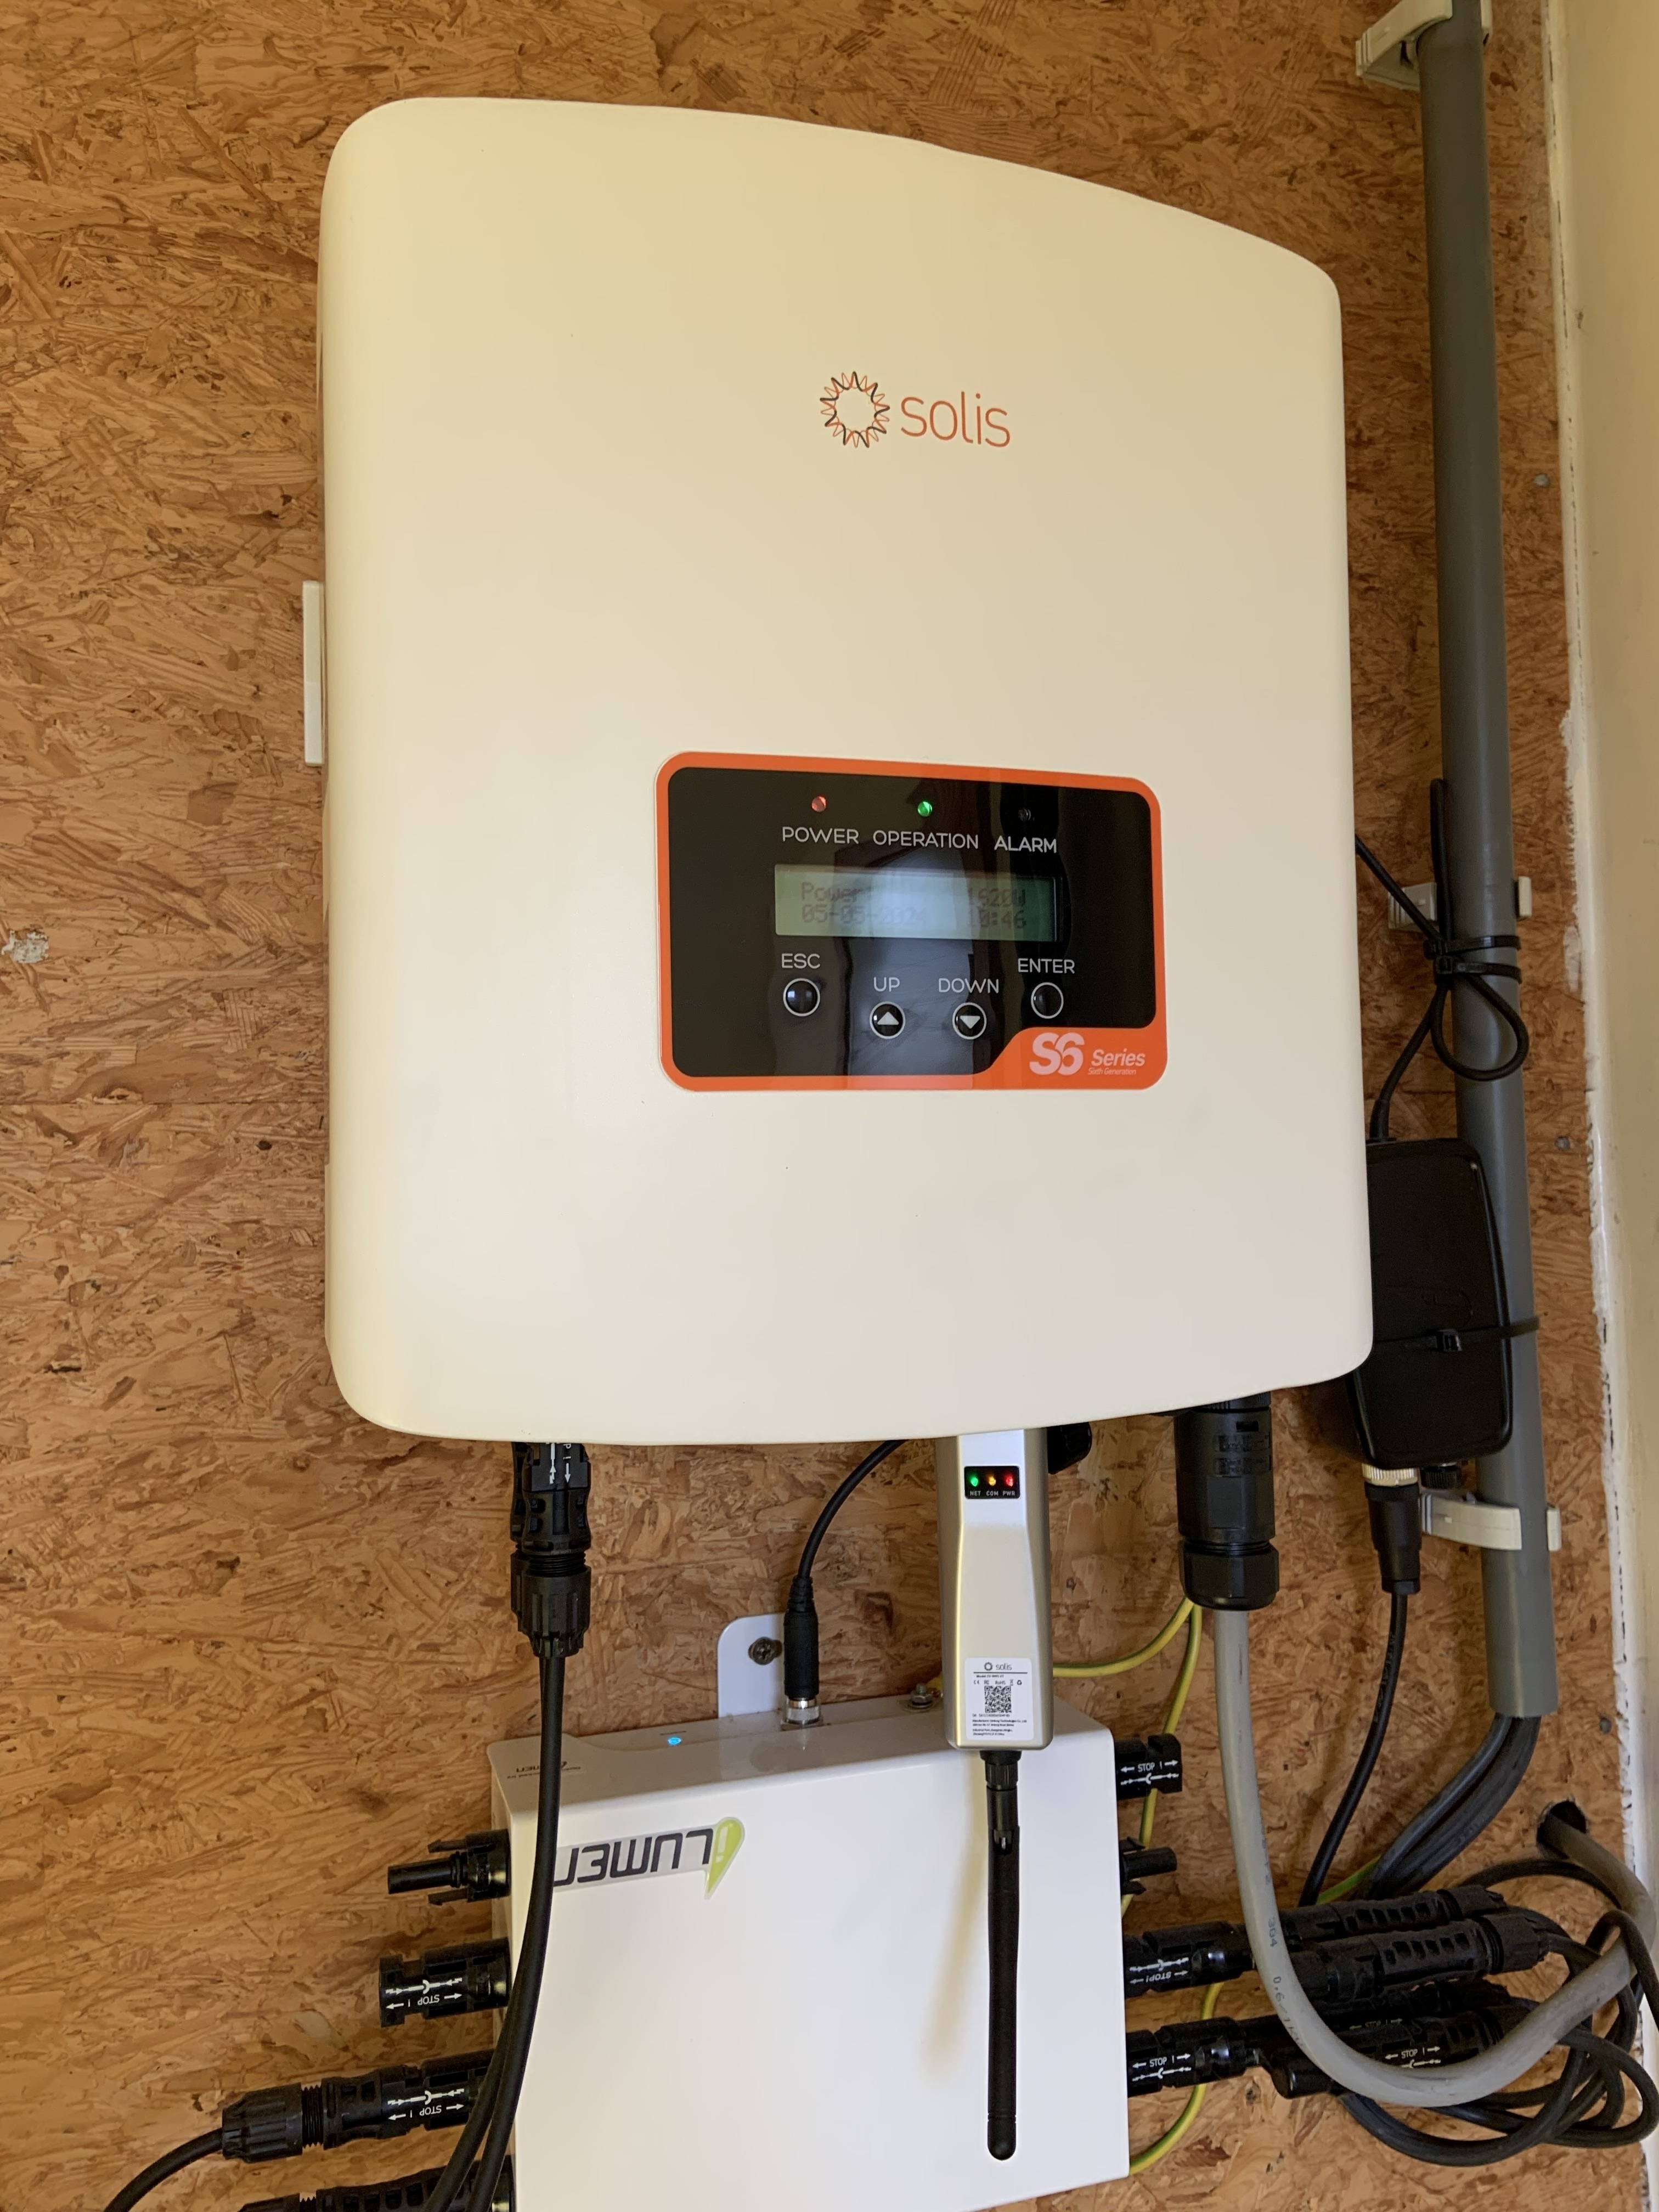
\includegraphics[width=7cm]{Omvormer} \hspace{0.5cm}
    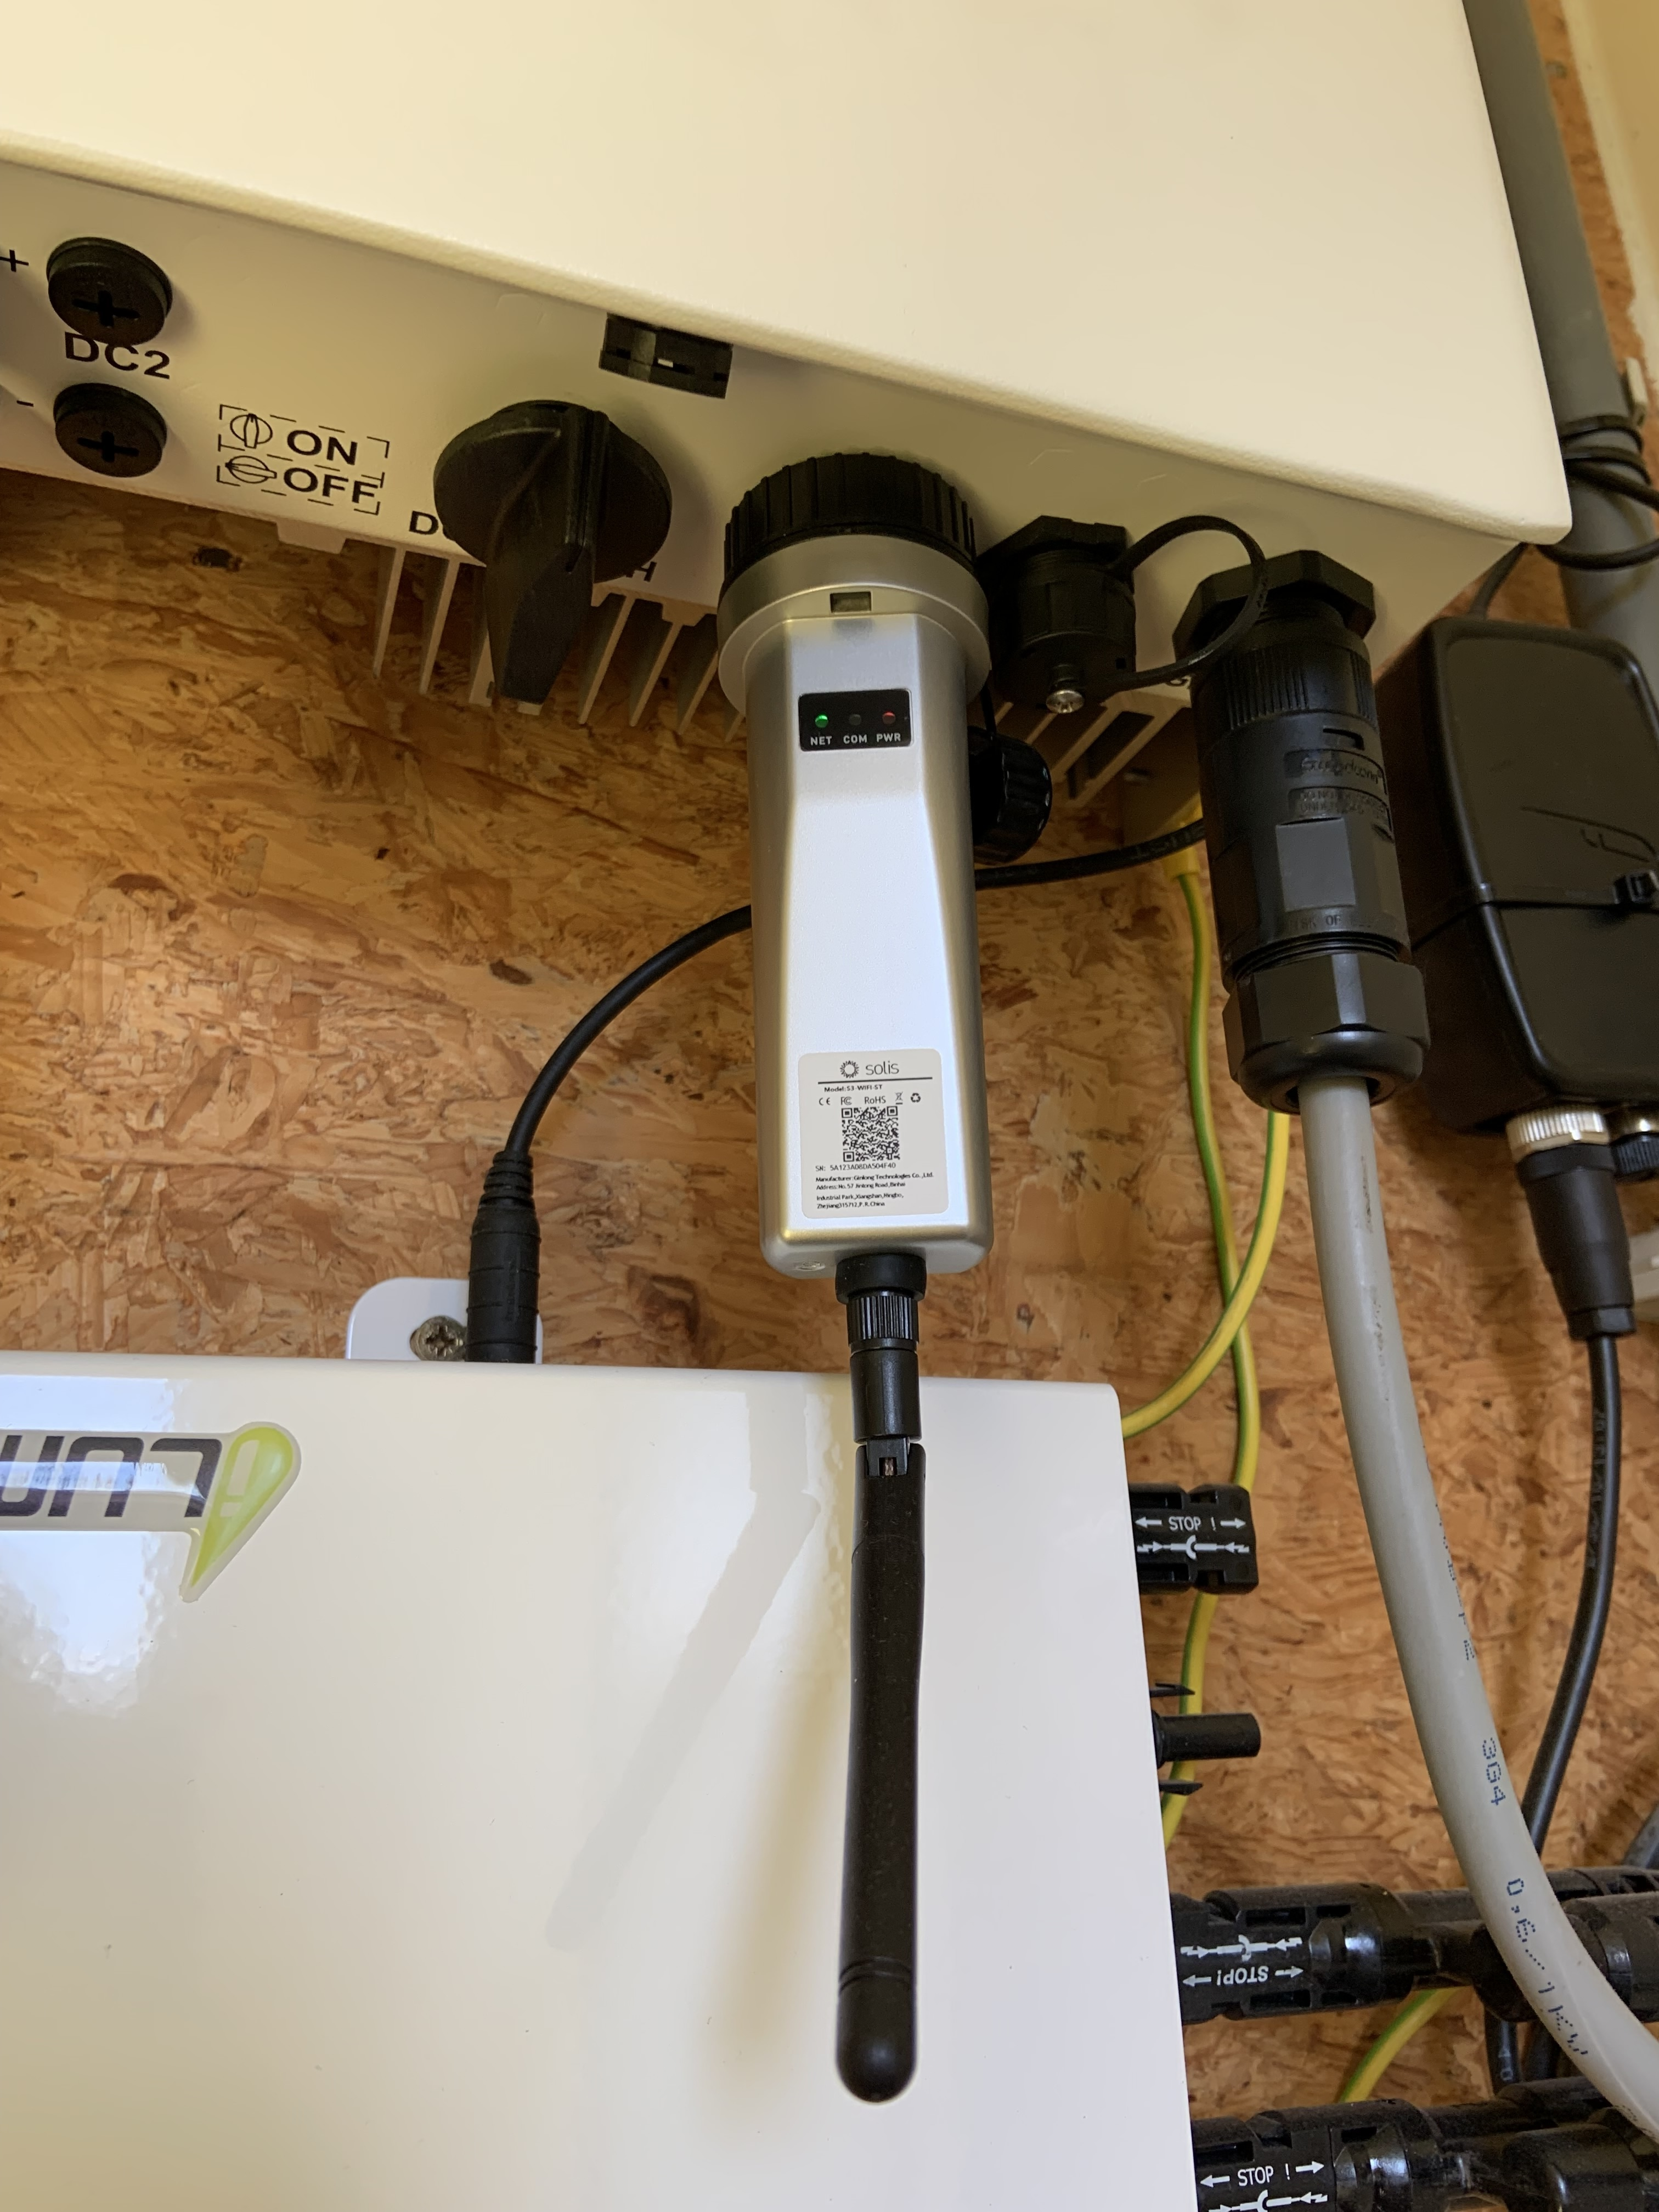
\includegraphics[width=7cm]{Wifi_Stick}
    \caption{Omvormer van de zonnepanelen met een wifi-stick.}
\end{figure}

Ook de data van de omvormer worden via het Python script weggeschreven naar een aparte InfluxDB databank en opgezet als een achtergrond service via de systeem manager voor Linux 'systemctl/systemd'. Zo blijft ook dit script automatisch uitgevoerd worden.

\subsection{\IfLanguageName{dutch}{Stroomproductie van zonnepanelen voorspellen met XGBoost}{Predicting power production PV system with XGBoost}}%
\label{sec:Stroomproductie van zonnepanelen voorspellen met XGBoost}

Het oorspronkelijke idee was om de stroomproductie van de zonnepanelen te gaan voorspellen op basis van de historische data van die stroomproductie. Voor dit onderzoek was er echter geen of slechts beperkte historische data voorhanden, omdat de metingen van de omvormer van de zonnepanelen pas gestart zijn bij het begin van het onderzoek. Na uitgebreid literatuuronderzoek werd beslist om de stroomproductie van de zonnepanelen te gaan voorspellen op basis van de hoeveelheid zonnestraling  \autocite{Sehrawat2023}, \autocite{Ledmaoui2023}, \autocite{Wang2022} en \autocite{Sansine2023}. Via de CAMS Radiation Service (CRS) van de Copernicus Atmosphere Monitoring Service (\href{https://atmosphere.copernicus.eu}{CAMS}) kan voldoende betrouwbare historische data met betrekking tot zonnestraling verkregen worden.

\subsubsection{Historische zonnestralingsdata verzamelen}

De zonnestralingsdata die via de CAMS Radiation Service (CRS) kan bekomen worden omvat tijdreeksen van globale, directe en diffuse instraling voor een tijdspanne van 1 februari 2004 tot en met 2 dagen geleden. De granulariteit van de data varieert van 1 maand tot 1 minuut en kan via een API-request opgevraagd worden. \\

Er bestaat een open-source Python library 'pvlib' \autocite{Jensen2023} die ontwikkeld werd om de opbrengst van zonnepanelen te simuleren. Deze library bevat ook tools om zonnestralingsdata op te vragen, waaronder de data van de CAMS Radiation Service (CRS). Omdat de reeds ontwikkelde scripts voor het uitlezen van de digitale elektriciteitsmeter en de omvormer van de zonnepanelen in Python geschreven zijn, worden ook de andere scripts in Python geschreven en kan de pvlib-library dus gebruikt worden. Om de zonnestralingsgegevens op te vragen moeten een aantal parameters worden meegegeven, waaronder de locatie (lengte- en breedtegraad), de start- en einddatum en de tijdsgranulariteit. Omdat van de gebruiker van de app niet kan verwacht worden dat hij of zij de geografische coördinaten van zijn of haar woning kent, wordt de Python library Geopy gebruikt om het ingevoerde adres van een gebruiker om te zetten in de correcte lengte- en breedgraad  coördinaten en deze vervolgens mee te geven in de API-call naar de CRS. \\

Voor dit onderzoek wordt de zonnestralingsdata voor een periode van iets meer dan 5 jaar opgevraagd, van 1 januari 2019 tot op heden om precies te zijn. Dat heden is evenwel de datum van 2 dagen eerder, aangezien het 2 dagen duurt vooraleer de CRS de waargenomen zonnestralingsdata verwerkt en opgeslagen heeft. Dit geeft voldoende data om via een machine learning algoritme de toekomstige hoeveelheid zonnestraling te gaan voorspellen. Voor de granulariteit werd geopteerd voor metingen om de 15 minuten. Zo zijn de metingen van de bekomen dataset voldoende gedetailleerd om accurate voorspellingen te kunnen maken, zonder dat de performantie in het gedrang komt. Bij metingen van 1 minuut blijkt de dataset te omvangrijk om er op een efficiënte en dus snelle manier berekeningen op uit te voeren.

\begin{figure}[h!]
    \centering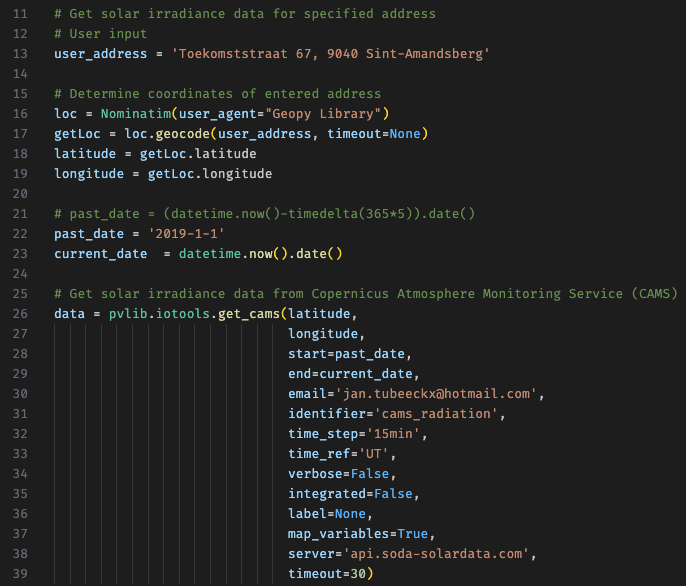
\includegraphics[scale=0.6]{Solar_Irradiance}
    \caption{\label{fig:Solar_Irradiance}Script voor het opvragen van de zonnestralingsdata.}
\end{figure} 

\newpage
\subsubsection{Weerdata}

Niet alleen de hoeveelheid zonnestraling is bepalend voor de stroomproductie van zonnepanelen, ook de weersomstandigheden oefenen een invloed uit. Vooral de omgevingstemperatuur, de relatieve luchtvochtigheid en de bewolkingsgraad zijn factoren die de stroomproductie van zonnepanelen kunnen vergroten of verkleinen \autocite{Sehrawat2023}. \\

Om de voorspelling van de toekomstige stroomproductie van de zonnepanelen accurater te maken, zal de zonnestralingsdata in de eerste plaats gecombineerd worden met historische weerdata voor dezelfde periode, van 1 januari 2019 tot op heden. Ook hiervoor werd gezocht naar een open-source API, waarmee de data via een Python script kan worden opgevraagd. Finaal is voor \href{https://dev.meteostat.net/}{Meteostat} gekozen. Deze API biedt een Pyhon library waarmee met slechts een enkele HTTP-request historische weerdata voor een bepaalde locatie kan worden opgevraagd. Meteostat verzamelt historische weer- en klimaatdata van weerstations en verschillende nationale meteorologische instituten van over de hele wereld. Omdat ook voor deze API-call de lengte- en breedtegraad van de gevraagde locatie moet worden ingegeven, wordt opnieuw gebruik gemaakt van de Python library Geopy waarmee een adres kan worden omgezet in de correcte lengte- en breedgraad coördinaten. \\

\begin{figure}[h!]
    \centering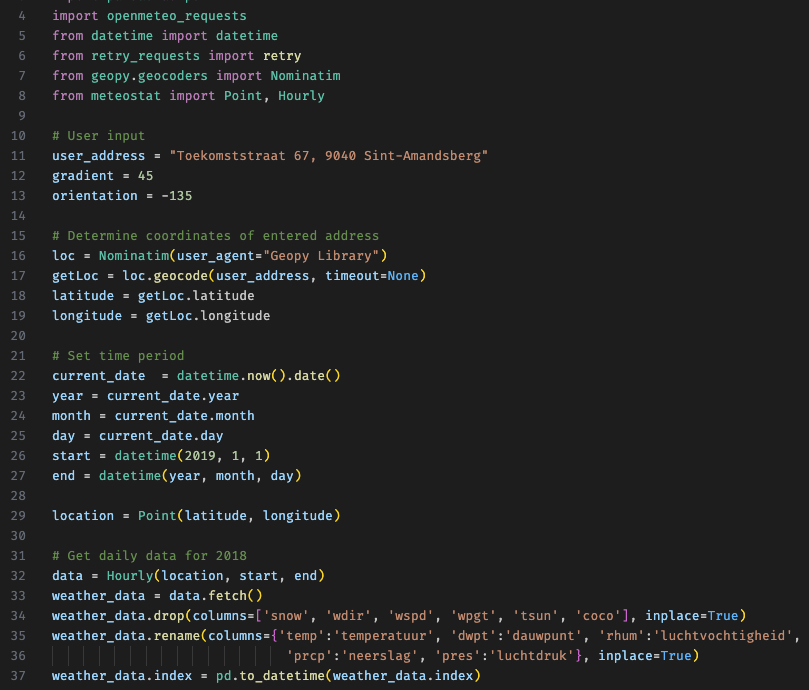
\includegraphics[scale=0.5]{Weerdata}
    \caption{\label{fig:Weerdata}Script voor het opvragen van de weerdata.}
\end{figure} 

Om de voorspelling van de stroomproductie van de zonnepanelen nog beter te maken, zal de bekomen voorspelling gecombineerd worden met de weersvoorspellingen voor de voorspelde periode. Aangezien Meteostat enkel historische data aanbiedt, moest een andere open-source weer-API gevonden worden. \href{https://open-meteo.com/}{Open-Meteo API} werkt ook samen met verschillende nationale meteorologische diensten waardoor het betrouwbare weersvoorspellingen aanbiedt. De aangeboden API-request is makkelijk in te stellen, zodat enkel de benodigde weerdata kan worden opgevraagd. Zo kan de data snel opgevraagd worden. Voor dit onderzoek worden enkel de voorspellingen van de omgevingstemperatuur, de relatieve luchtvochtigheid en de bewolkingsgraad opgehaald.

\subsubsection{Voorspelling met XGBoost}

Door het toenemend belang van hernieuwbare energie is er al heel wat onderzoek verricht naar het voorspellen van de elektriciteitsproductie van PV-systemen door toepassing van machine learning. Uit de meest recente onderzoeken blijkt dat Extreem Gradient Boosting (XGBoost) andere machine learning algoritmes overtreft bij het voorspellen van historische zonnestraling  \autocite{Ledmaoui2023}, \autocite{Wang2022} en \autocite{BarreraAnimas2022}. Om die reden wordt voor dit onderzoek gebruik gemaakt van XGBoost om de toekomstige zonnestraling en vervolgens de stroomproductie van zonnepanelen te voorspellen. \\

De dataset die als invoer voor het XGBoost algoritme gebruikt werd, is dus een combinatie van historische zonnestralingsdata en weerdata. Deze datset werd eerst gezuiverd van anomalieën door alle negatieve en ontbrekende waarden te verwijderen, anders zouden deze fouten de voorspelde waarden kunnen vertekenen. Na het opschonen van de data werden bestaande correlaties onderzocht. Hiervoor werd de Python library 'Seaborn' gebruikt, waarmee een heatmap van de correlaties tussen de verschillende kenmerken van de dataset kon worden opgemaakt. Daaruit blijkt inderdaad dat vooral de omgevingstemperatuur (positief) en luchtvochtigheid (negatief) het sterkst correleren met de globale horizontale instraling van de zon (GHI). 

\begin{figure}[h!]
    \centering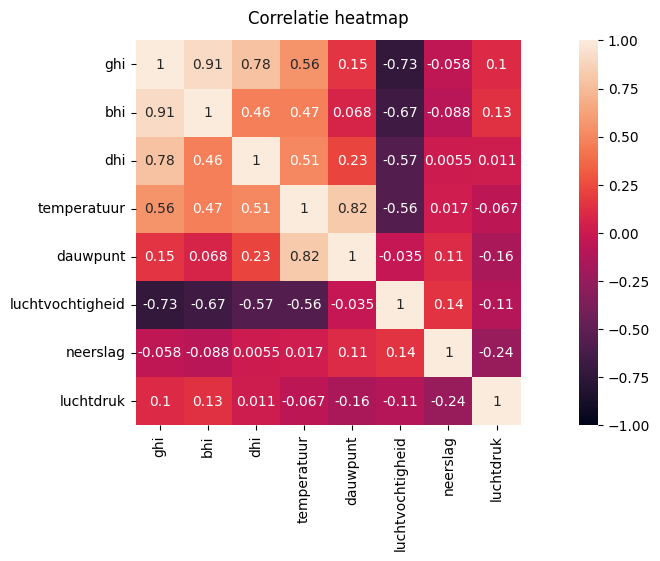
\includegraphics[scale=0.7]{correlatie}
    \caption{\label{fig:correlatie}Heatmap van correlaties tussen de verschillende kenmerken van de dataset.}
\end{figure} 

\newpage
De historische zonnestralingsdata die gebruikt wordt, kan beschouwd worden als tijdreeksen (time-series) vermits de data geordend is volgens een tijdsindex. Om tijdreeksen te kunnen voorspellen, moeten deze eerst worden omgezet in 'supervised learning' problemen, van gewone reeksen naar paren van invoer en uitvoer reeksen. Door de omzetting naar een bepaalde invoer X en uitvoer y, kan een algoritme leren hoe de uitvoerpatronen uit de invoerpatronen kunnen voorspeld worden. De omzetting naar een  'supervised learning' probleem gebeurt door de toevoeging van zogenaamde features of numerieke kenmerken op basis van de datum van elk datapunt van de dataset die als invoer voor de voorspelling gebruikt wordt. \\

\begin{figure}[h!]
    \centering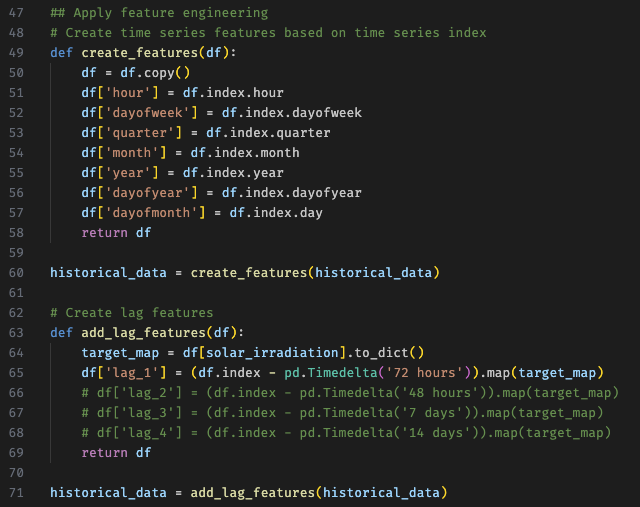
\includegraphics[scale=0.6]{Features_Lags}
    \caption{\label{fig:Features_Lags}Screenshot van de Python code voor het aanmaken van features en lags.}
\end{figure} 

\subsection{\IfLanguageName{dutch}{Weergave uitgelezen data en voorspelling met een iOS app}{Display of data and prediction with an iOS app}}%
\label{sec:Weergave uitgelezen data en voorspelling met een iOS app}

Omdat een smartphone makkelijker en vaker consulteerbaar is, werd in dit onderzoek geopteerd voor de ontwikkeling van een mobiele app om de elektriciteitsconsumptie- en productie weer te geven en op te volgen. De app is ontwikkeld voor iOS omdat dit het testen vergemakkelijkt. De iOS-app werd gebouwd in de geïntegreerde ontwikkelomgeving (IDE) XCode met SwiftUI en UIKit. Voor documentatie en tutorials werd gebruik gemaakt van het \href{https://developer.apple.com/}{Apple developer platform}. \\

\begin{figure}[h!]
    \centering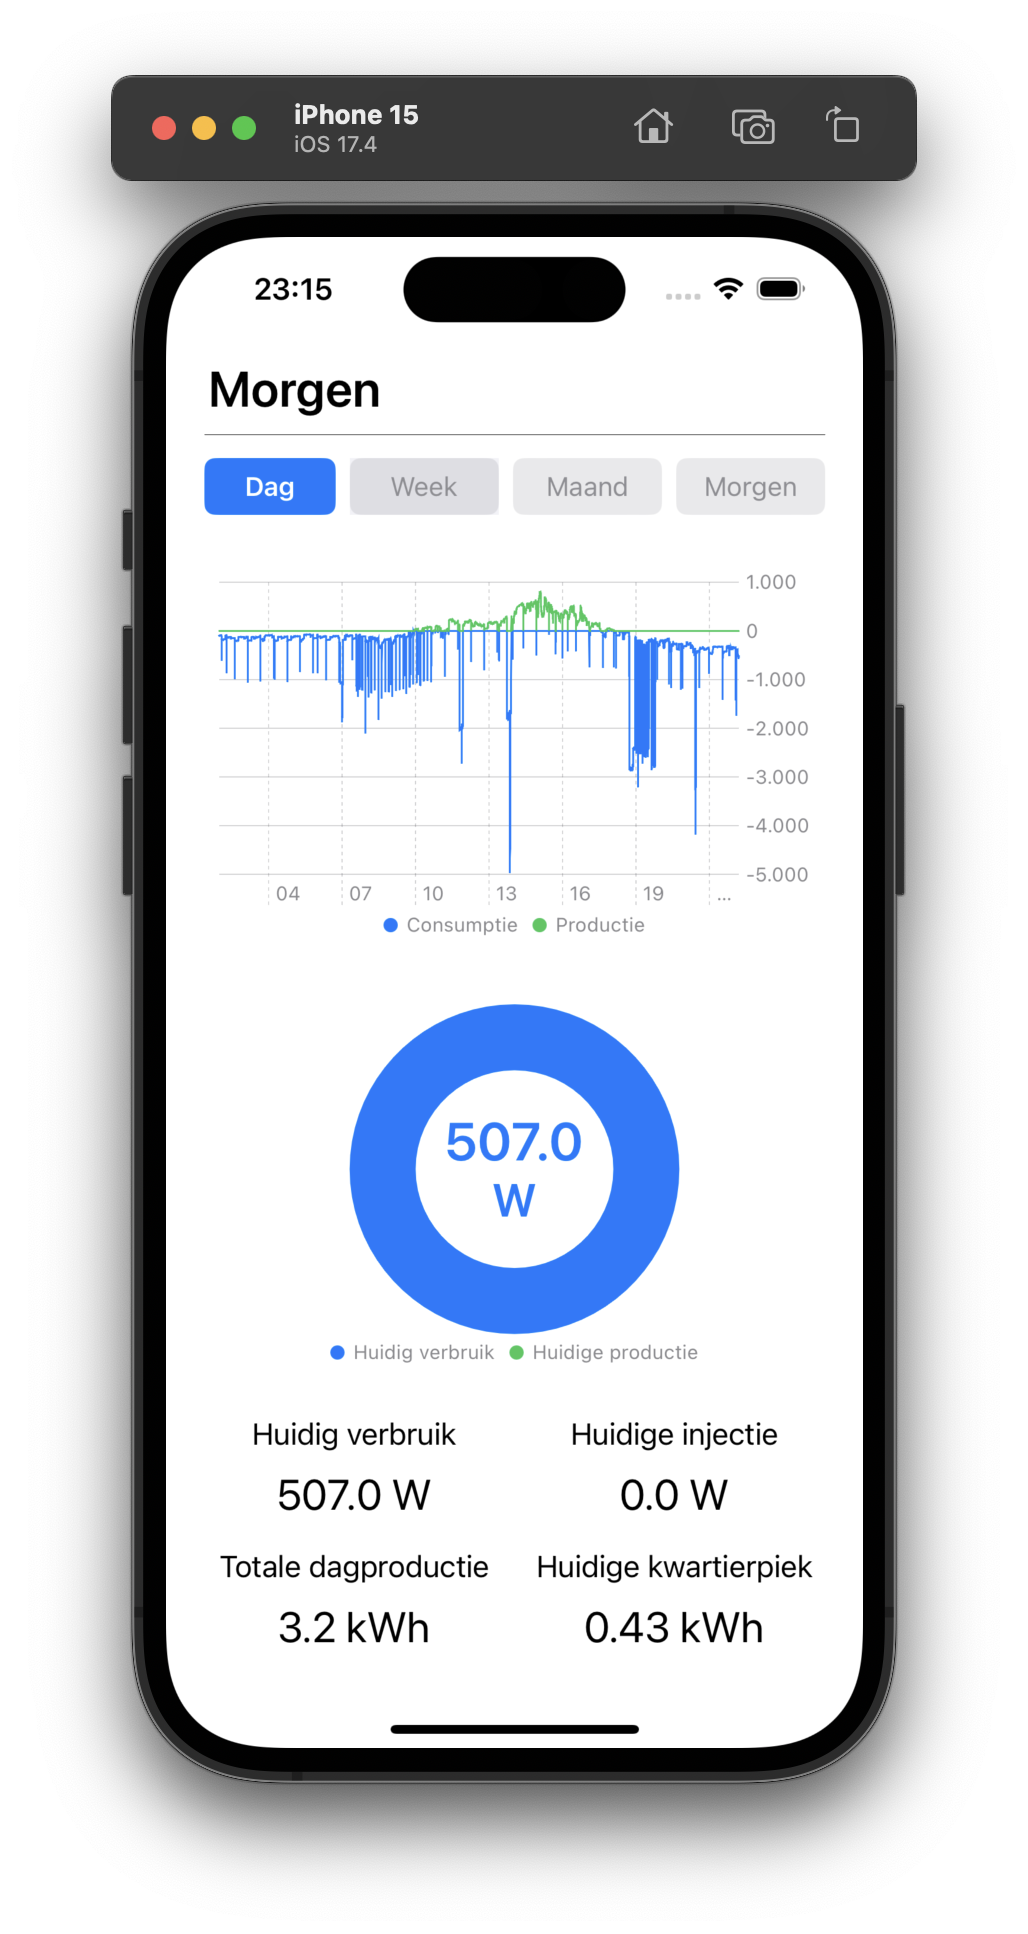
\includegraphics[scale=0.4]{Iphone_Dag}
    \caption{\label{fig:Iphone_Dag}Screenshot dagweergave.}
\end{figure} 


\subsection{\IfLanguageName{dutch}{Aansturing slimme stekkers op basis van voorspelde stroomproductie}{Predicting power production PV system with XGBoost}}%
\label{sec:Aansturing slimme stekkers aansturen op basis van voorspelde stroomproductie}

De eerste slimme toestellen die via de app zullen worden beheerd zijn zonnepanelen en een warmtepomp \autocite{Uytterhoeven2019}. Door de afschaffing van de virtueel terugdraaiende teller voor eigenaars van zonnepanelen, waarbij de teller van de elektriciteitsmeter terugdraait wanneer meer elektriciteit wordt opgewekt dan verbruikt, kan het verlies van dit voordeel opgevangen door het verbruik van de warmtepomp te laten samenvallen met de productiemomenten van de zonnepanelen \autocite{Selleslagh2021}. Wanneer echter uit de weersverwachtingen blijkt dat er een aanzienlijke elektriciteitsproductie zal zijn, zal de app  mede op basis van historiek van het elektriciteitsverbruik automatisch ook andere toestellen, zoals de vaatwas of wasmachine gaan inschakelen.

 Om de sanitaire toestellen te kunnen gaan inschakelen, zal in de eerste plaats gekeken worden of deze toestellen van zichzelf reeds slim zijn. Meer concreet zal geverifieerd worden of ze over een Soft Real Time Operating System beschikken (Soft RTOS) en via het wifinetwerk kunnen communiceren met een app. Voor de sanitaire toestellen die niet slim zijn, zal gebruik gemaakt worden van slimme stopcontacten. Daarbij wordt er tussen het klassieke stopcontact en de stekker van het toestel een apparaat geplaatst, waardoor een toestel op een eenvoudige manier slim kan gemaakt worden \autocite{Jong2020}.

\chapter{Conclusie}%
\label{ch:Conclusie}